\documentclass[
    12pt,
    a4paper,
    ngerman,
    color=3b,% Farbe für Hervorhebungen auf Basis der Deklarationen in den
    %type=intern,
    %titlepage=true,
    marginpar=false,
    colorback=false,
    %logo=head,
    leqno,
]{tudaexercise}
\usepackage{import}
% Import all Packages from Main Preamble with relative Path
\subimport*{../../}{preamble}
% Get Labels from Main Document using the xr-hyper Package
\externaldocument{../../AuD-Zusammenfassung-2020}
% Set Graphics Path, so pictures load correctly
\graphicspath{{../../}}


\begin{document}
\section{Grundlegende Datenstrukturen}\index{Grundlegende Datenstrukturen}
\subsection{Stacks}\label{Stacks}\index{Stacks}
\begin{itemize}
    \item \fatsf{Abstrakter Datentyp Stack}
          \begin{itemize}
              \item \texttt{new S()}
                    \begin{itemize}
                        \item Erzeugt neuen (leeren) Stack
                    \end{itemize}
              \item \texttt{s.isEmpty()}
                    \begin{itemize}
                        \item Gibt an, ob Stack \texttt{s} leer ist
                    \end{itemize}
              \item \texttt{s.pop()}
                    \begin{itemize}
                        \item Gibt oberstes Element vom Stack \texttt{s} zurück und löscht es vom Stack
                        \item Gibt Fehlermeldung aus, falls der Stack leer ist
                    \end{itemize}
              \item \texttt{s.push(k)}
                    \begin{itemize}
                        \item Schreibt \texttt{k} als neues oberstes Element auf Stack \texttt{s}
                    \end{itemize}
              \item Abstrakter Aufbau:
                    \begin{itemize}
                        \item \fatsf{LIFO}-Prinzip - Last in, First out
                        \item[] 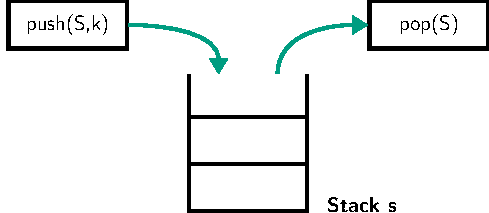
\includegraphics[width=6cm]{pictures/LIFO/lifo}
                    \end{itemize}
          \end{itemize}

    \item \fatsf{}{Beispiel Bitcoin}\index{Bitcoin}
    \item[] 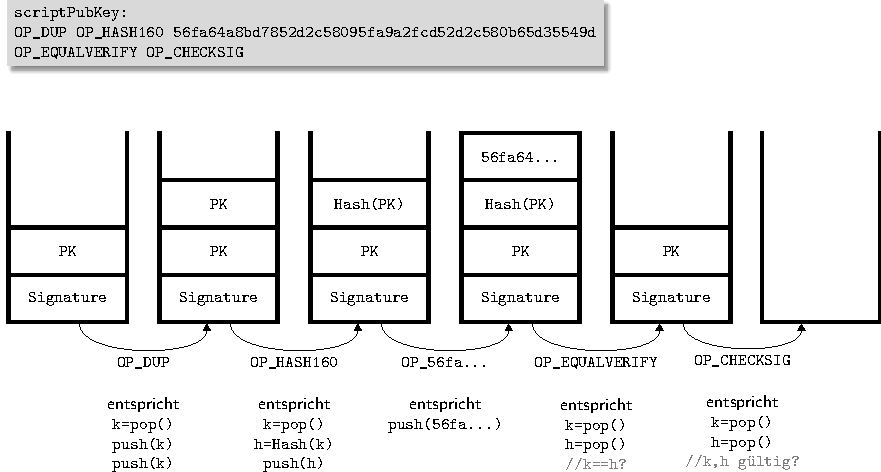
\includegraphics[width=15cm]{pictures/bitcoin_stack_example/bitcoin_stack_example}
          \clearpage
    \item \fatsf{Stacks als Array}
          \begin{itemize}
              \item[] 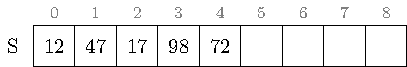
\includegraphics[]{pictures/staack_als_array/stack_als_array}
              \item \texttt{s.top} zeigt immer auf oberstes Element
              \item \texttt{pop()} führt dazu, dass \texttt{s.Top} sich eins nach links bewegt
              \item \texttt{push(k)} führt dazu, dass \texttt{s.Top} sich eins nach rechts bewegt
          \end{itemize}

    \item \fatsf{Stacks als Array - Methoden, falls maximale Größe bekannt}\\
          \begin{minipage}[t]{.4\textwidth}
              \begin{codeBlock}[autogobble]{title=new(S)}
                  S.A[]=ALLOCATE(MAX);
                  S.top=-1;
              \end{codeBlock}
          \end{minipage}
          \begin{minipage}[t]{.4\textwidth}
              \begin{codeBlock}[autogobble]{title=isEmpty(S)}
                  IF S.top<0 THEN
                    return true;
                  ELSE
                    return false;
              \end{codeBlock}
          \end{minipage}
          \\
          \begin{minipage}[t]{.4\textwidth}
              \begin{codeBlock}[autogobble]{title=pop(S)}
                  IF isEmpty(S) THEN
                    error "underflow";
                  ELSE
                    s.top=s.top-1;
                    return S.A[S.top+1];
              \end{codeBlock}
          \end{minipage}
          \begin{minipage}[t]{.4\textwidth}
              \begin{codeBlock}[autogobble]{title=push(S)}
                  IF S.top==MAX-1 THEN
                    error "overflow";
                  ELSE
                    S.top=S.top+1;
                    S.A[S.top]=k;
              \end{codeBlock}
          \end{minipage}
          %\item[] 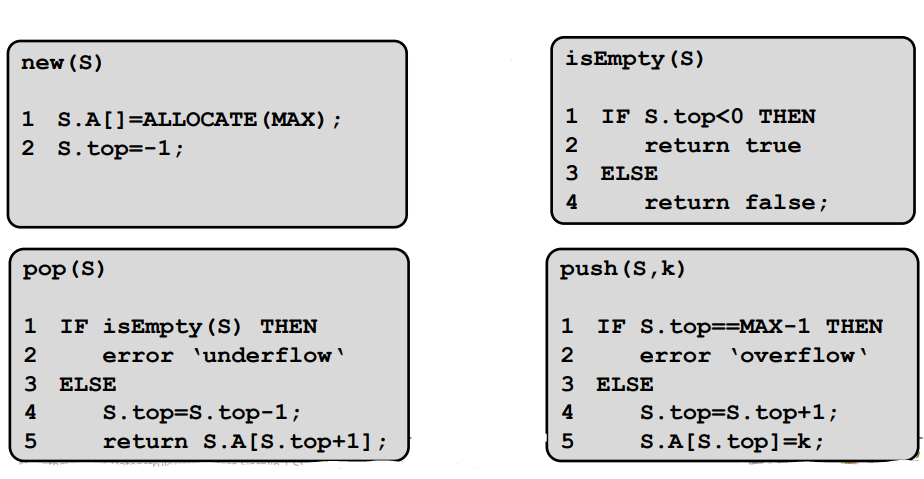
\includegraphics[width=12cm]{pictures/arrayMethods1}

    \item \fatsf{Stacks mit variabler Größe - Einfach}
          \begin{itemize}
              \item Falls \texttt{push(k)} bei vollem Array $\Rightarrow$ Vergößerung des Arrays
              \item Erzeugen eines neuen Arrays mit Länge + 1 und Umkopieren aller Elemente
              \item Durchschnittlich $\Omega(n)$ Kopierschritte pro \texttt{push}-Befehl
          \end{itemize}
          \clearpage
    \item \fatsf{Stacks mit variabler Größe - Verbesserung}
          \begin{itemize}
              \item Idee:
                    \begin{itemize}
                        \item Wenn Grenze erreicht, Verdopplung des Speichers und Kopieren der Elemente
                        \item Falls weniger als ein Viertel belegt, schrumpfe das Array wieder
                    \end{itemize}
              \item Methoden:
              \item[] \texttt{RESIZE(A,m)} reserviert neuen Speicher der Grö\ss e \texttt{m} und kopiert \texttt{A} um\\
                    \begin{minipage}[t]{.5\textwidth}
                        \begin{codeBlock}[autogobble]{title=new(S)}
                            S.A[]=ALLOCATE(1);
                            S.top=-1;
                            S.memsize=1;
                        \end{codeBlock}
                    \end{minipage}
                    \begin{minipage}[t]{.4\textwidth}
                        \begin{codeBlock}[autogobble]{title=isEmpty(S)}
                            IF S.top<0 THEN
                                return true;
                            ELSE
                                return false;
                        \end{codeBlock}
                    \end{minipage}
                    \\
                    \begin{minipage}[t]{.5\textwidth}
                        \begin{codeBlock}[autogobble]{title=pop(S)}
                            IF isEmpty(S) THEN
                                error "underflow";
                            ELSE
                                S.top=S.top-1;
                                IF 4*(S.top+1)==S.memsize THEN
                                    S.mensize=s.memsize/2;
                                    RESIZE(S.A,S.memsize);
                                return S.A[S.top+1];
                        \end{codeBlock}
                    \end{minipage}
                    \begin{minipage}[t]{.4\textwidth}
                        \begin{codeBlock}[autogobble]{title=push(S)}
                            S.top=S.top+1;
                            S.A[S.top]=k;
                            IF S.top+1>=S.memsize THEN
                                S.memsize=2*S.memsize;
                                RESIZE(S.A,S.memsize);
                        \end{codeBlock}
                    \end{minipage}
                    %\item[] 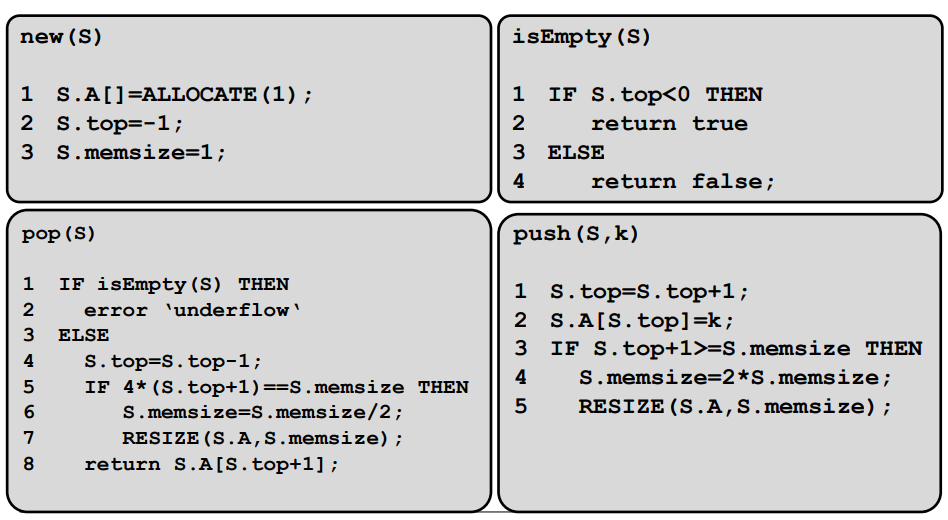
\includegraphics[width=12cm]{pictures/stacksArray2.PNG}

              \item Im Durchschnitt für jeder der mindestens \texttt{n} Befehle $\Theta(1)$ Umkopierschritte

          \end{itemize}
\end{itemize}

\pagebreak
\subsection{Verkettete Listen}\label{Verkettete Listen}\index{Verkettete Listen}
\begin{itemize}
    \item \fatsf{Aufbau}
          \begin{itemize}
              \item[] 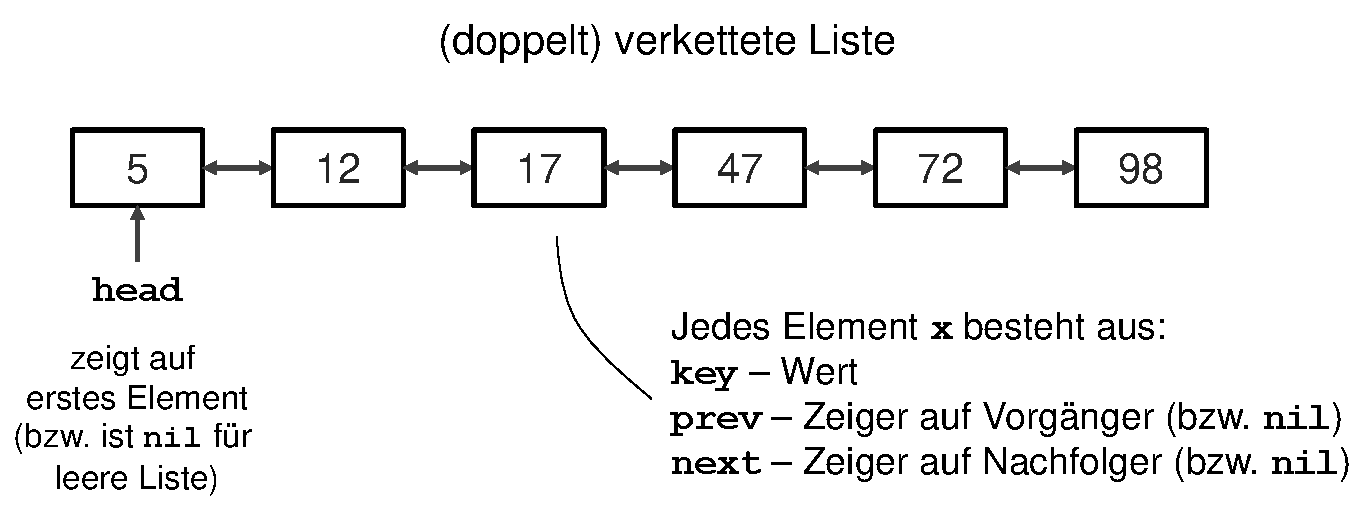
\includegraphics[width=12cm]{pictures/linkedList1.pdf}
          \end{itemize}

    \item \fatsf{Verkettete Listen durch Arrays}
          \begin{itemize}
              \item[] Entspricht doppelter Verkettung zwischen 45 und 12
              \item[] 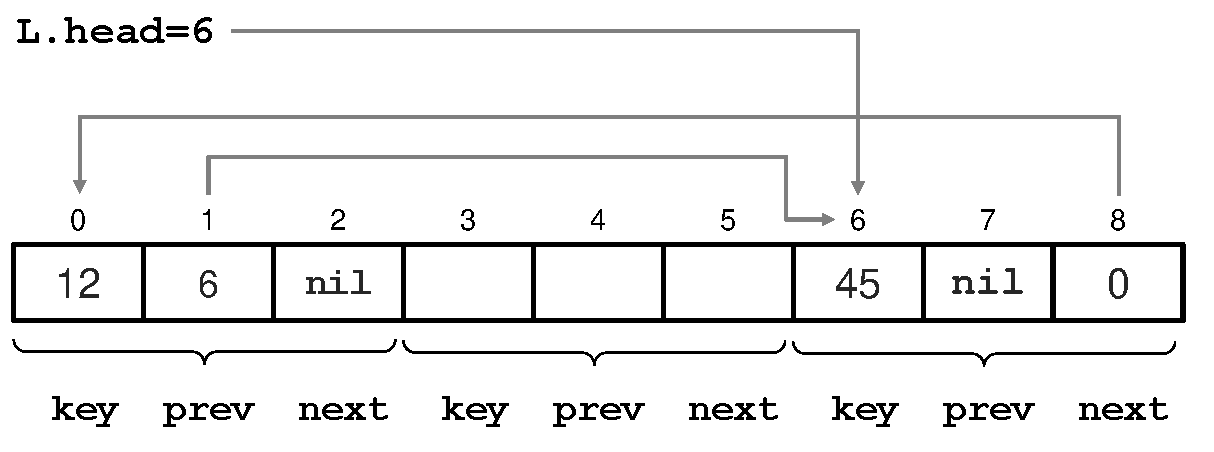
\includegraphics[width=12cm]{pictures/linkedList2.pdf}
          \end{itemize}

    \item \fatsf{Elementare Operationen auf Listen}
          \begin{itemize}
              \item \textit{Suche nach Element}
                    \begin{itemize}
                        \item Laufzeit beträgt im Worst Case $\Theta(n)$
                        \item[] $\Rightarrow$ Keine Überprüfung, ob Wert bereits in Liste, sonst $\Theta(n)$
                        \item Code:
                        \item[]
                              \begin{codeBlock}[autogobble]{title={search(L,k) // Returns pointer to k in L (or nil)}}
                                  current = L.head;
                                  WHILE current != nil AND current.key != k DO
                                    current = current.next;
                                  return current;
                              \end{codeBlock}
                        \item[] 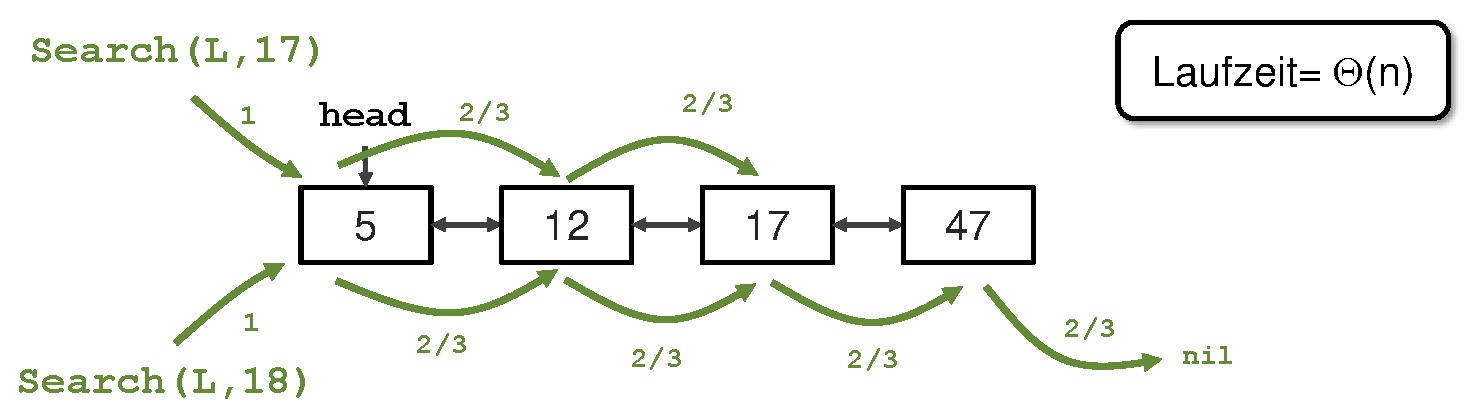
\includegraphics[width=12cm]{pictures/verketteteListenSuche.pdf}
                    \end{itemize}

                    \clearpage
              \item \textit{Einfügen eines Elements am Kopf der Liste}
                    \begin{itemize}
                        \item Laufzeit beträgt $\Theta(1)$, da Einfügen am Kopf
                        \item Code:
                        \item[]
                              \begin{codeBlock}[autogobble]{title={insert(L,x)}}
                                  insert(L,x)
                                  x.next = l.head;
                                  x.prev = nil;
                                  IF L.head != nil THEN
                                    L.head.prev = x;
                                  L.head = x;
                              \end{codeBlock}
                    \end{itemize}

              \item \textit{Löschen eines Elements aus Liste}
                    \begin{itemize}
                        \item Laufzeit beträgt $\Theta(1)$, da hier Pointer auf Objekt gegeben
                        \item[] Löschen eines Wertes $k$ mithilfe von Suche beträgt $\Omega(n)$
                        \item Code:
                        \item[]
                              \begin{codeBlock}[autogobble]{title={delete (L,x)}}
                                  IF x.prev != nil THEN
                                    x.prev.next = x.next
                                  ELSE
                                    L.head = x.next;
                                  IF x.next != nil THEN
                                    x.next.prev = x.prev;
                              \end{codeBlock}
                    \end{itemize}
          \end{itemize}

    \item \fatsf{Vereinfachung per Wächter/Sentinels}\index{Sentinel}
          \begin{itemize}
              \item Ziel ist die Eliminierung der Spezialfälle für Listenanfang/-ende
              \item[] 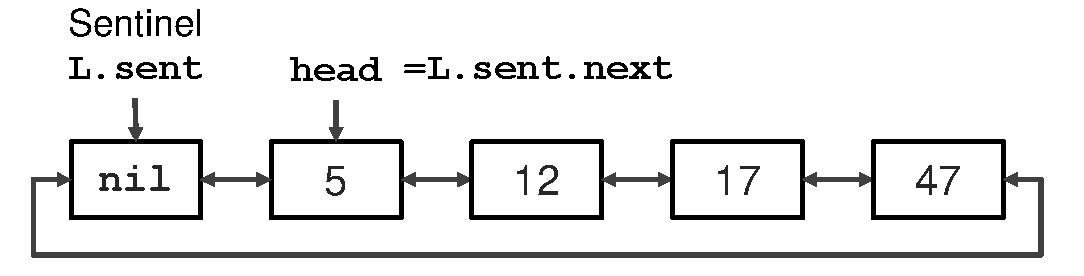
\includegraphics[width=12cm]{pictures/linkedListSentinel.pdf}
              \item Löschen mit Sentinels:
              \item[]
                    \begin{codeBlock}[autogobble]{title={deleteSent(L,x)}}
                        x.prev.next = x.next;
                        x.next.prev = x.prev;
                    \end{codeBlock}
          \end{itemize}
\end{itemize}
\clearpage
\subsection{Queues}\label{Queues}\index{Queue}
\begin{itemize}
    \item \textbf{Abstrakter Datentyp Queue}
          \begin{itemize}
              \item \texttt{new Q()}
                    \begin{itemize}
                        \item Erzeuge neue (leere) Queue
                    \end{itemize}

              \item \texttt{q.isEmpty()}
                    \begin{itemize}
                        \item Gibt an, ob Queue \texttt{q} leer ist
                    \end{itemize}

              \item \texttt{q.dequeue()}
                    \begin{itemize}
                        \item Gibt vorderstes Element aus \texttt{q} zurück und löscht es auf Queue
                        \item Fehlermeldung, falls Queue leer ist
                    \end{itemize}

              \item \texttt{q.enqueue(k)}
                    \begin{itemize}
                        \item Schreibt \texttt{k} als neues hinterstes Element auf \texttt{q}
                        \item Fehlermeldung, falls Queue voll ist
                    \end{itemize}

              \item Abstrakter Aufbau:
                    \begin{itemize}
                        \item \fatsf{FIFO}-Prinzip\index{FIFO} / First in, First out
                        \item[] 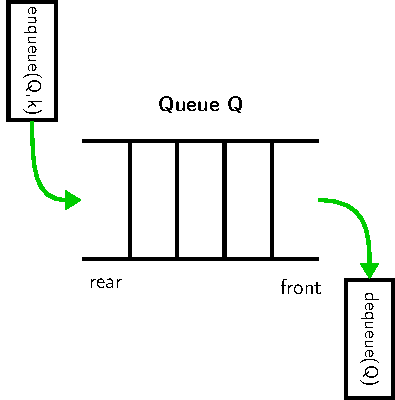
\includegraphics[width=8cm]{pictures/FIFO/FIFO}
                    \end{itemize}
          \end{itemize}

          \pagebreak

    \item \fatsf{Queues als (virtuelles) zyklisches Array}\index{zyklisches Array}
          \begin{itemize}
              \item[] Bekannt: Maximale Elemente gleichzeitig in Queue
              \item[] 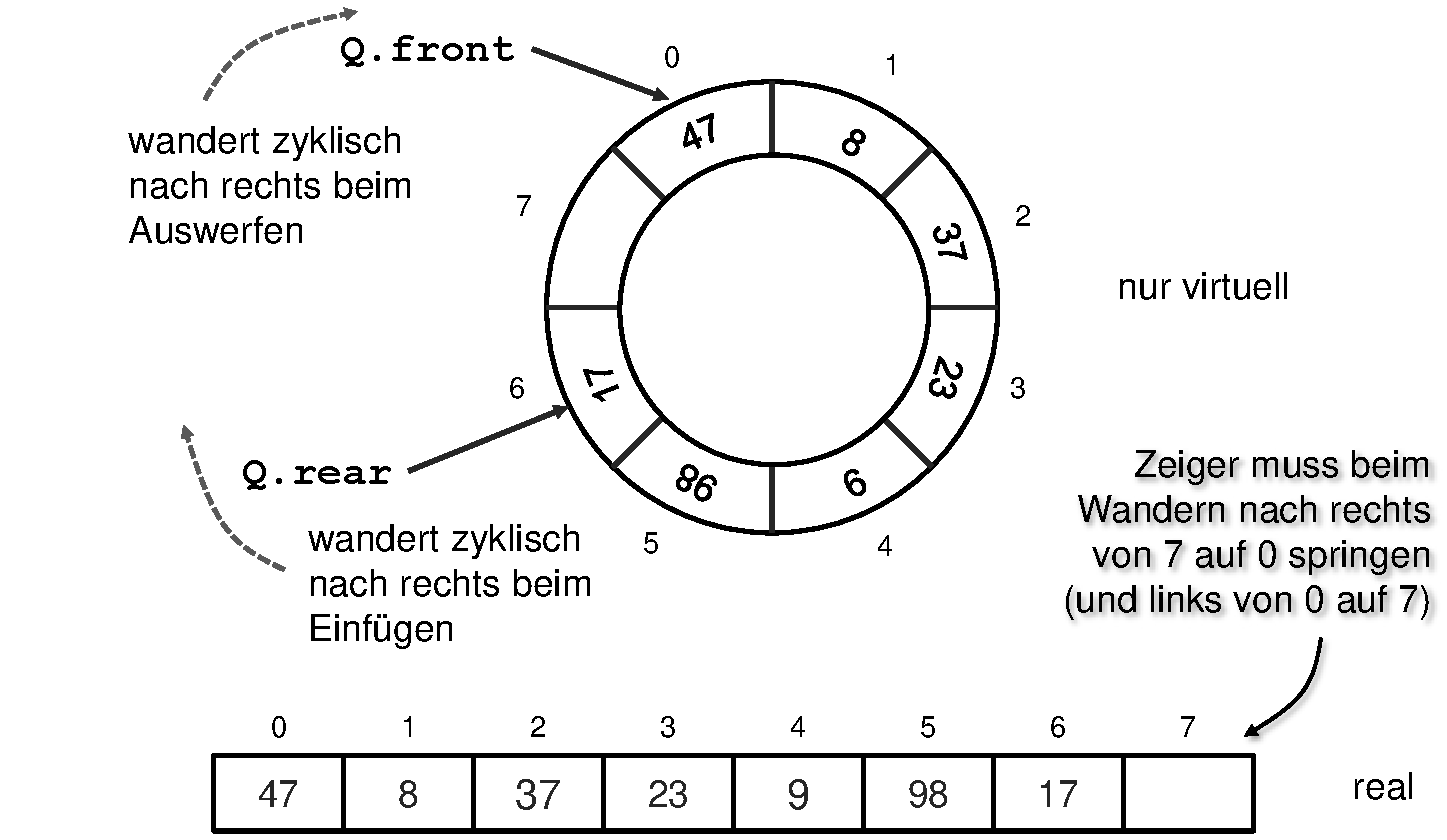
\includegraphics[width=12cm]{pictures/queueZyklisch.pdf}
              \item[]
              \item Problem, falls \texttt{Q.rear} und \texttt{Q.front} auf selbes Element zeigen
                    \begin{itemize}
                        \item Speichere Information, ob Schlange leer oder voll, in boolean \texttt{empty}
                        \item Alternativ: Reserviere ein Element des Arrays als Abstandshalter
                    \end{itemize}

              \item Methoden für zyklisches Array\\
                    \begin{minipage}[t]{.45\textwidth}
                        \begin{codeBlock}[autogobble]{title={new(Q)}}
                            Q.A[]=ALLOCATE(MAX);
                            Q.front=0;
                            Q.rear=0;
                            Q.empty=true;
                        \end{codeBlock}
                    \end{minipage}
                    \begin{minipage}[t]{.45\textwidth}
                        \begin{codeBlock}[autogobble]{title={isEmpty(Q)}}
                            return Q.empty;
                        \end{codeBlock}
                    \end{minipage}
                    \\
                    \begin{minipage}[t]{.45\textwidth}
                        \begin{codeBlock}[autogobble]{title={dequeue(Q)}}
                            IF isEmpty(Q) THEN
                                error "underflow";
                            ELSE
                                Q.front=Q.front+1 mod MAX;
                                IF Q.front==Q.rear THEN
                                    Q.empty=true;
                                return Q.A[Q.front-1 mod MAX];
                        \end{codeBlock}
                    \end{minipage}
                    \begin{minipage}[t]{.45\textwidth}
                        \begin{codeBlock}[autogobble]{title={enqueue(Q,k)}}
                            IF Q.rear==Q.front AND !Q.isEmpty
                            THEN error "overflow";
                            ELSE
                                Q.A[Q.rear]=k;
                                Q.rear=Q.rear+1 mod MAX;
                                Q.empty=false;
                        \end{codeBlock}
                    \end{minipage}
                    %\item[] 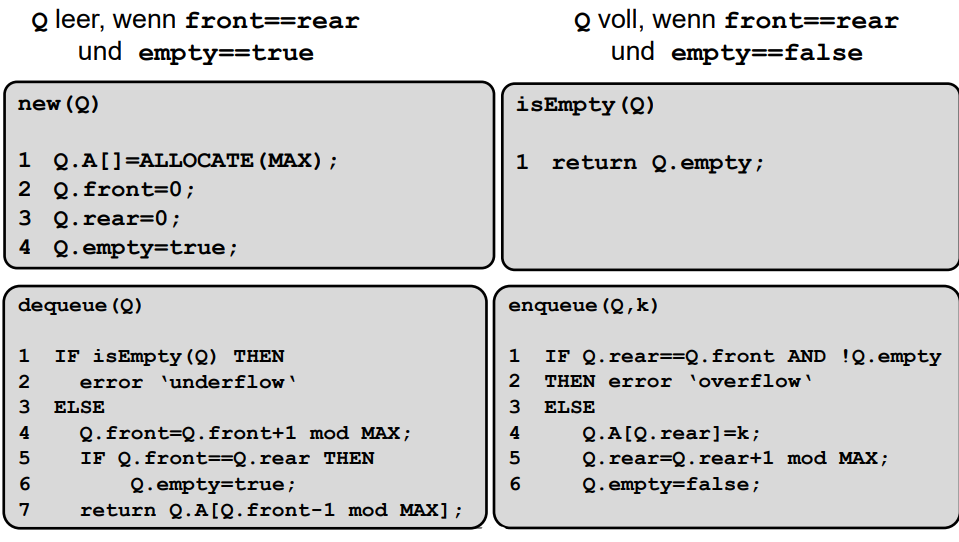
\includegraphics[width=12cm]{pictures/queueZyklischM.PNG}
          \end{itemize}

          \pagebreak

    \item \textbf{Queues durch einfach verkettete Listen}
          \begin{itemize}
              \item[] 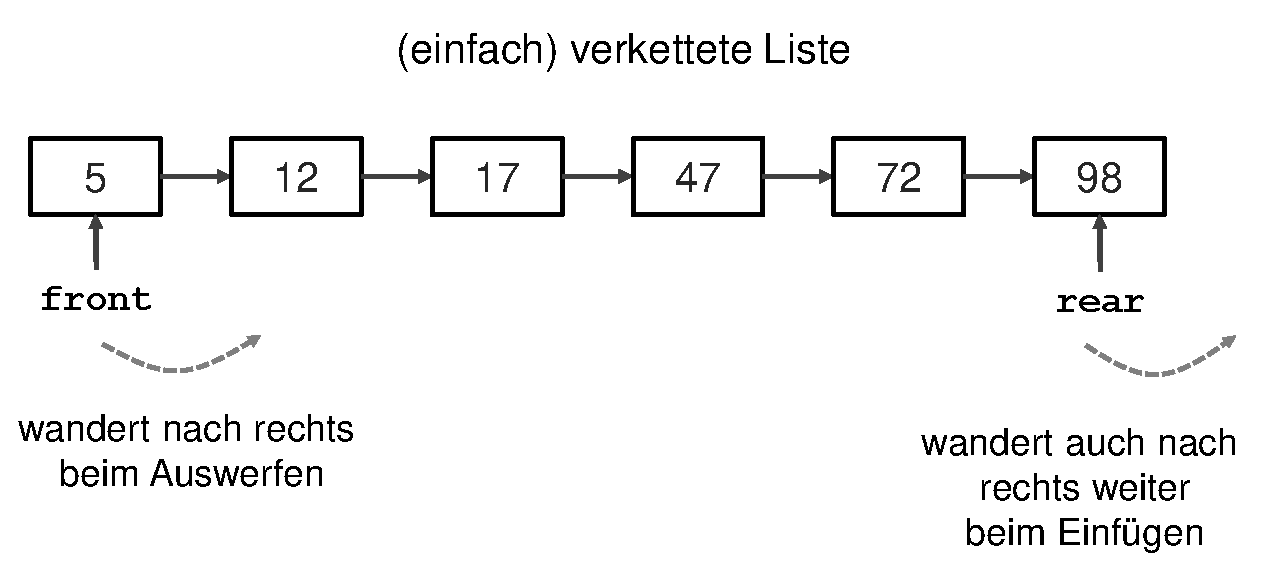
\includegraphics[width=12cm]{pictures/queuesListe1.pdf}
              \item[] Methoden:
              \item[] %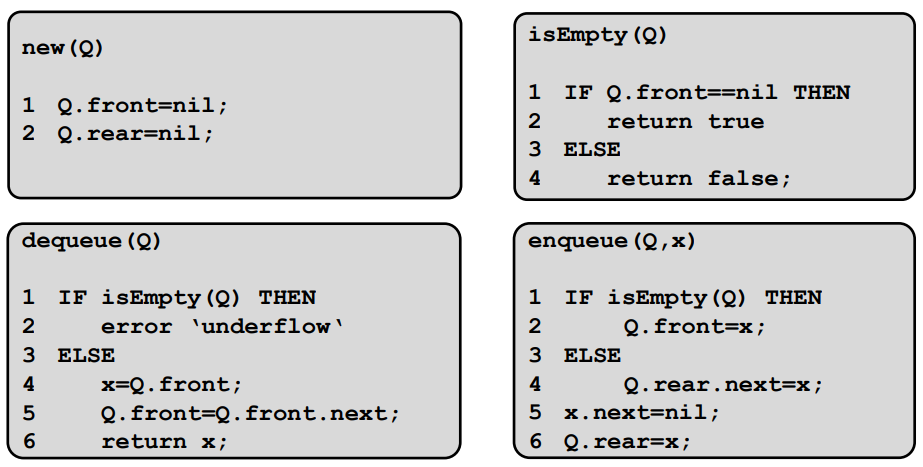
\includegraphics[width=12cm]{pictures/queuesListe2.PNG} 
                    \begin{minipage}[t]{.4\textwidth}
                        \begin{codeBlock}[autogobble]{title={new(Q)}}
                            Q.front=nil;
                            Q.rear=nil;
                        \end{codeBlock}
                    \end{minipage}
                    \begin{minipage}[t]{.4\textwidth}
                        \begin{codeBlock}[autogobble]{title={isEmpty(Q)}}
                            IF Q.front==nil THEN
                                return true;
                            ELSE
                                return false;
                        \end{codeBlock}
                    \end{minipage}
                    \\
                    \begin{minipage}[t]{.4\textwidth}
                        \begin{codeBlock}[autogobble]{title={dequeue(Q)}}
                            IF isEmpty(Q) THEN
                                error "underflow";
                            ELSE
                                x=Q.front;
                                Q.front=Q.front.next;
                                return x;
                        \end{codeBlock}
                    \end{minipage}
                    \begin{minipage}[t]{.4\textwidth}
                        \begin{codeBlock}[autogobble]{title={enqueue(Q,k)}}
                            IF isEmpty(Q) THEN
                                Q.front=x;
                            ELSE
                                Q.rear.next=x;
                            x.next=nil;
                            Q.rear=x;
                        \end{codeBlock}
                    \end{minipage}
          \end{itemize}

    \item \fatsf{Laufzeit}
          \begin{itemize}
              \item Enqueue: $\Theta(1)$
              \item Dequeue: $\Theta(1)$
          \end{itemize}
\end{itemize}

\pagebreak
\subsection{Binäre Bäume}\label{Binaere Baeume}\index{Binäre Bäume}
\begin{itemize}
    \item \fatsf{Bäume durch verkettete Listen}
          \begin{itemize}
              \item[] \includegraphics[width=12cm]{pictures/binäreBaumeListe.PNG}
              \item[] Bäume sind "`azyklisch"'(also "`keine Schleifen zwischen Knoten"')
          \end{itemize}

    \item \fatsf{Darstellung als (ungerichteter) Graph}
          \begin{itemize}
              \item[]
                    \begin{minipage}[t]{0.45\textwidth}
                        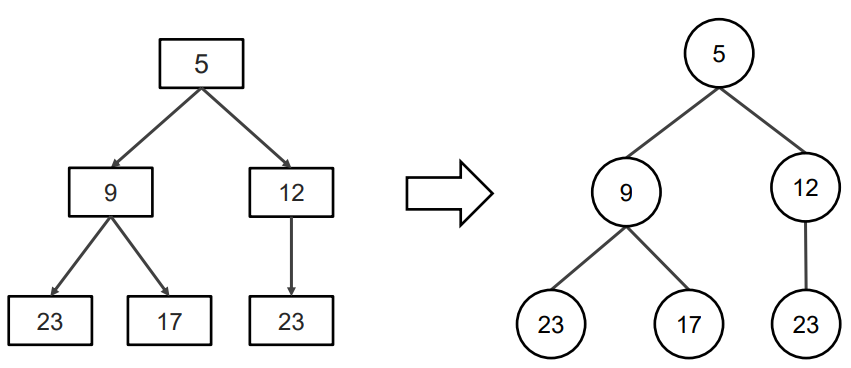
\includegraphics[width=7cm]{pictures/baumGraph1.PNG}
                    \end{minipage}
                    \begin{minipage}[t]{0.45\textwidth}
                        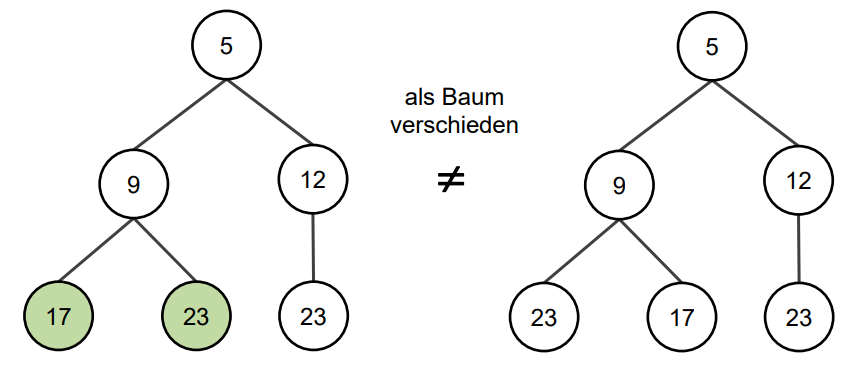
\includegraphics[width=7cm]{pictures/baumGraph2.PNG}
                    \end{minipage}
          \end{itemize}

    \item \fatsf{Allgemeine Begrifflichkeiten}\index{Vorfahre}\index{ancestor}\index{Wurzel}\index{root}\index{parent}\index{Elternknoten}\index{Kindknoten}\index{child}\index{Geschwisterknoten}\index{sibling}\index{Nachkomme}\index{descendant}\index{Blatt}\index{leaf}\index{Höhe (Baum)}
          \begin{itemize}
              \item[]
                    \begin{minipage}[t]{0.45\textwidth}
                        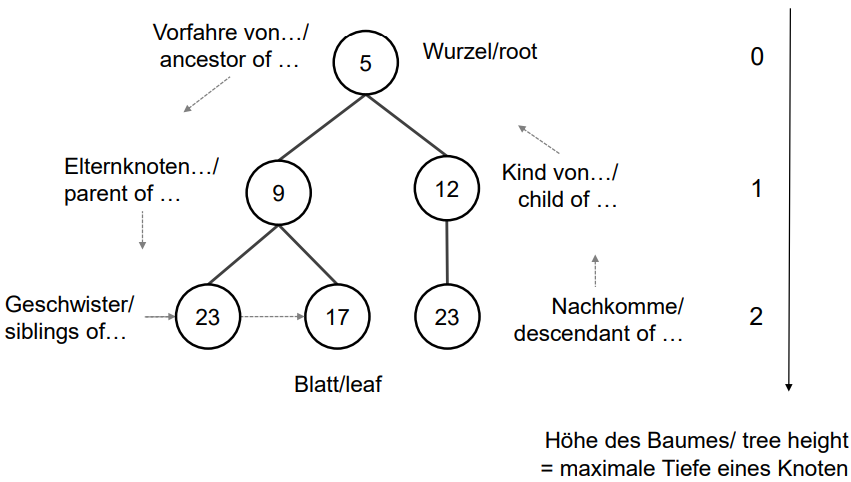
\includegraphics[width=8cm]{pictures/baumBegriffe1.PNG}
                    \end{minipage}
                    \begin{minipage}[t]{0.45\textwidth}
                        \vspace{-3.5cm}
                        \begin{itemize}
                            \item Blatt: Knoten ohne Nachfolger
                            \item Nachkomme von x: \\
                                  Erreichbar durch Pfad ausgehend von x
                        \end{itemize}
                    \end{minipage}
          \end{itemize}
          \clearpage
    \item \fatsf{Begrifflichkeiten Binärbaum}
          \begin{itemize}
              \item[]\index{Halbblatt}\index{Teilbaum}
                    \begin{minipage}[t]{0.45\textwidth}
                        \includegraphics[width=8cm]{pictures/binärbaumBegriffe}
                    \end{minipage}
                    \begin{minipage}[t]{0.45\textwidth}
                        \vspace{-4.5cm}
                        \begin{itemize}
                            \item Jeder Knoten hat maximal zwei Kinder \\
                                  \texttt{left=child[0]} und \texttt{right=child[1]}
                            \item Ausgangsgrad jedes Knoten ist $\leq 2$
                            \item Höhe leerer Baum per Konvention $-1$
                            \item Hohe (nicht-leerer) Baum: \\
                                  max\{Höhe aller Teilbäume der Wurzel\} + 1
                            \item Halbblatt: Knoten mit nur einem Kind
                        \end{itemize}
                    \end{minipage}
          \end{itemize}


    \item \fatsf{Traversieren von Bäumen}\index{Traversieren von Bäumen}
          \begin{itemize}
              \item Darstellung eines Baumes mithilfe einer Liste der Werte aller Knoten
              \item Laufzeit bei $n$ Knoten: $T(n) = O(n)$
              \item Nutzung der Preorder für das Kopieren von Bäumen
                    \begin{enumerate}
                        \item Preorder betrachtet Knoten und legt Kopie an
                        \item Preorder geht dann in Teilbäume und kopiert diese
                    \end{enumerate}
              \item Nutzung der Postorder für das Löschen von Bäumen
                    \begin{enumerate}
                        \item Postorder geht zuerst in Teilbäume und löscht diese
                        \item Betrachten des Knoten erst danach und dann Löschung dieses
                    \end{enumerate}
              \item[]
              \item[]
                    \begin{minipage}[t]{0.4\textwidth}
                        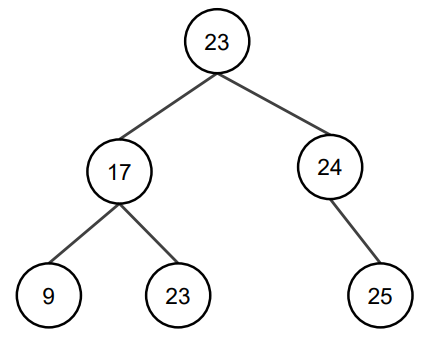
\includegraphics[width=6cm]{pictures/inorder1}
                    \end{minipage}
                    \begin{minipage}[t]{0.5\textwidth}
                        \vspace{-4.75cm}
                        \begin{itemize}
                            \item[] 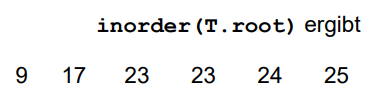
\includegraphics[width=6cm]{pictures/inorder2}
                            \item[] 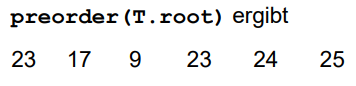
\includegraphics[width=6cm]{pictures/preorder1}
                            \item[] 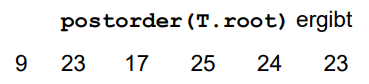
\includegraphics[width=6cm]{pictures/postorder1}
                        \end{itemize}
                    \end{minipage}
              \item[]
              \item[] \textbf{Code:} \index{inorder}\index{preorder}\index{postorder}\\
                    \begin{minipage}[t]{0.29\textwidth}
                        \begin{codeBlock}[autogobble]{title={inorder(x)}}
                            IF x != nil THEN
                                inorder(x.left);
                                print x.key;
                                inorder(x.right);
                        \end{codeBlock}
                    \end{minipage}
                    \begin{minipage}[t]{0.3\textwidth}
                        \begin{codeBlock}[autogobble]{title={preorder(x)}}
                            IF x != nil THEN
                                print x.key;
                                preorder(x.left);
                                preorder(x.right);
                        \end{codeBlock}
                    \end{minipage}
                    \begin{minipage}[t]{0.31\textwidth}
                        \begin{codeBlock}[autogobble]{title={postorder(x)}}
                            IF x != nil THEN
                                postorder(x.left);
                                postorder(x.right);
                                print x.key;
                        \end{codeBlock}
                    \end{minipage}
          \end{itemize}
          \clearpage
    \item \fatsf{Eindeutige Bestimmbarkeit von Bäumen}
          \begin{itemize}
              \item Nur In-, Pre-, Postorder reichen nicht zur eindeutigen Bestimmbarkeit von Bäumen
              \item[] $\Rightarrow$ Preorder/Postorder $+$ Inorder $+$ eindeutige Werte sind notwendig
              \item[] 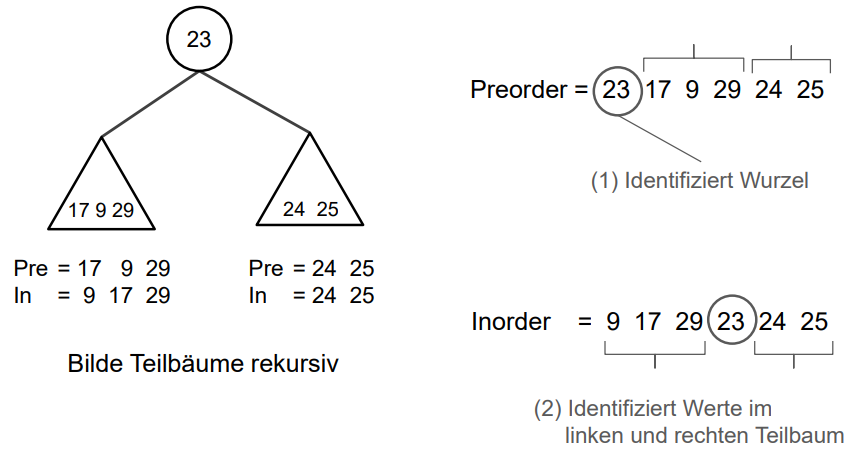
\includegraphics[width=12cm]{pictures/bestimmbarkeitBaum.PNG}
          \end{itemize}


    \item \fatsf{Abstrakter Datentyp Baum}
          \begin{itemize}
              \item \textit{Abstrakter Aufbau:}
                    \begin{itemize}
                        \item \texttt{new T()}
                              \begin{itemize}
                                  \item Erzeugt neuen Baum namens \texttt{t}
                              \end{itemize}

                        \item \texttt{t.search(k)}
                              \begin{itemize}
                                  \item Gibt Element \texttt{x} in Baum \texttt{t} mit \texttt{x.key == k} zurück
                              \end{itemize}

                        \item \texttt{t.insert(k)}
                              \begin{itemize}
                                  \item Fügt Element \texttt{x} in Baum \texttt{t} hinzu
                              \end{itemize}

                        \item \texttt{t.delete(x)}
                              \begin{itemize}
                                  \item Löscht \texttt{x} aus Baum \texttt{t}
                              \end{itemize}
                    \end{itemize}

              \item \textit{Suche nach Elementen:}
                    \begin{itemize}
                        \item Laufzeit = $\Theta(n)$ (Jeder Knoten maximal einmal, jeder Knoten im schlechtesten Fall)
                        \item Starte mit \texttt{search(T.root,k)}
                        \item Code:
                        \item[]
                              \begin{codeBlock}[autogobble]{title={search(x,k)}}
                                  IF x == nil THEN return nil;
                                  IF x.key == k THEN return x;
                                  y = search(x.left,k);
                                  IF y != nil THEN return y;
                                  return search(x.right,k);
                              \end{codeBlock}
                    \end{itemize}
                    \clearpage
              \item \textit{Einfügen von Elementen:}
                    \begin{itemize}
                        \item Laufzeit = $\Theta(1)$
                        \item Hier wird als Wurzel eingefügt (Achtung: Erzeugt linkslastigen Baum)
                        \item Code:
                        \item[]
                              \begin{codeBlock}[autogobble]{title={insert(T,x) // x.parent == x.left == x.right == nil;}}
                                  IF T.root != nil THEN
                                    T.root.parent = x;
                                    x.left = T.root;
                                  T.root = x;
                              \end{codeBlock}
                    \end{itemize}

              \item \textit{Löschen von Elementen:}
                    \begin{itemize}
                        \item Laufzeit = $\Theta(h)$ (Höhe des Baumes, $h=n$ möglich)
                        \item Hier: Ersetze $x$ durch Halbblatt ganz rechts
                        \item[] \includegraphics[width=12cm]{pictures/löschenBaum.PNG}
                              \pagebreak
                        \item \texttt{Connect}-Algorithmus:
                        \item[]
                              \begin{minipage}[t]{0.35\textwidth}
                                  \includegraphics[width=5cm]{pictures/löschenBaumConnect.PNG}
                              \end{minipage}
                              \begin{minipage}[t]{0.45\textwidth}
                                  \vspace{-7cm}
                                  \begin{itemize}
                                      \item Laufzeit = $\Theta(1)$
                                      \item[]
                                            \begin{codeBlock}[autogobble]{title={connect(T,y,w) // Connects w to y.parent}}
                                                v = y.parent;
                                                IF y != T.root THEN
                                                    IF y == v.right THEN
                                                        v.right = w;
                                                    ELSE
                                                        v.left = w;
                                                ELSE
                                                    T.root = w;
                                                IF w != nil THEN
                                                    w.parent = v;
                                            \end{codeBlock}
                                  \end{itemize}
                              \end{minipage}

                        \item \texttt{Delete}-Algorithmus:
                        \item[]
                              \begin{minipage}{0.4\textwidth}
                                  \includegraphics[width=6cm]{pictures/löschenBaumDelete.PNG}
                              \end{minipage}
                              \begin{minipage}{0.45\textwidth}
                                  \begin{itemize}
                                      \item[]
                                            \begin{codeBlock}[autogobble]{title={delete(T,x) // assumes x in T}}
                                                y = T.root;
                                                WHILE y.right != nil DO
                                                    y = y.right;
                                                connect(T,y,y.left);
                                                IF x != y THEN
                                                    y.left = x.left;
                                                    IF x.left != nil THEN
                                                        x.left.parent = y;
                                                    y.right = x.right;
                                                    IF x.right != nil THEN
                                                        x.right.parent = y;
                                                    connect(T,x,y);
                                            \end{codeBlock}
                                  \end{itemize}
                              \end{minipage}
                    \end{itemize}
          \end{itemize}
\end{itemize}

\pagebreak
\subsection{Binäre Suchbäume}\label{Binaere Suchbaeume}\index{Binäre Suchbäume}
\begin{itemize}
    \item \fatsf{Definition}
          \begin{itemize}
              \item Totale Ordnung auf den Werten
              \item Für alle Knoten $z$ gilt:
              \item[] Wenn $x$ Knoten im linken Teilbaum von $z$, dann \texttt{x.key $\leq$ z.key}
              \item[] Wenn $y$ Knoten im rechten Teilbaum von $z$, dann \texttt{y.key $\geq$ z.key}
              \item Preorder/Postorder + eindeutige Werte $\Rightarrow$ Eindeutige Identifizierung
          \end{itemize}

    \item \fatsf{Suchen im Binären Suchbaum}
          \begin{itemize}
              \item[]
                    \begin{minipage}{0.4\textwidth}
                        \includegraphics[width=8cm]{pictures/binärerSuchbaumSuche.PNG}
                    \end{minipage}
                    \begin{minipage}{0.5\textwidth}
                        \begin{itemize}
                            \item Laufzeit $= O(h)$ (Höhe)
                            \item Code:
                            \item[]
                                  \begin{codeBlock}[autogobble]{title={search(x,k) // 1. Aufruf: x = root}}
                                      IF x == nil OR x.key == k THEN
                                        return x;
                                      IF x.key > k THEN
                                        return search(x.left,k);
                                      ELSE
                                        return search(x.right,k);
                                  \end{codeBlock}
                            \item Iterativer Code:
                            \item[]
                                  \begin{codeBlock}[autogobble]{title={iterative-search(x,k)}}
                                      WHILE x != nil AND x.key != k DO
                                        IF x.key > k THEN
                                            x = x.left;
                                        ELSE
                                            x = x.right;
                                      return x;
                                  \end{codeBlock}
                        \end{itemize}
                    \end{minipage}
          \end{itemize}
          \clearpage
    \item \fatsf{Einfügen im Binary Search Tree}
          \begin{itemize}
              \item[]
                    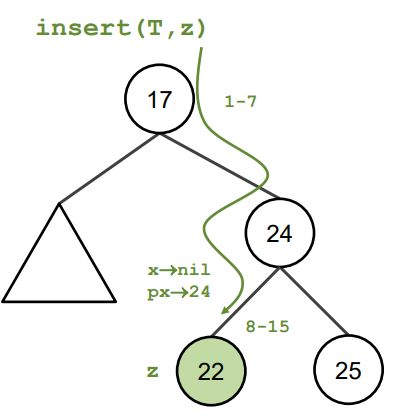
\includegraphics[width=8cm]{pictures/binärerSuchbaumEinfügen.PNG}
                    \begin{itemize}
                        \item Laufzeit = $O(h)$
                        \item Aufwendiger, da Ordnung erhalten werden muss
                        \item Code:
                        \item[]\label{BST-Insert}
                              \begin{codeBlock}[autogobble]{title={insert (T,z) // z.left == z.right == nil;}}
                                  x = T.root;
                                  px = nil;
                                  WHILE x != nil DO
                                    px = x;
                                    IF x.key > z.key THEN
                                        x = x.left;
                                    ELSE
                                        x = x.right;
                                  z.parent = px;
                                  IF px == nil THEN
                                    T.root = z;
                                  ELSE
                                    IF px.key > z.key THEN
                                        px.left = z;
                                    ELSE
                                        px.right = z;
                              \end{codeBlock}
                    \end{itemize}
          \end{itemize}

          \pagebreak

    \item \fatsf{Löschen im BST}
          \begin{itemize}
              \item \textit{Verschiedene Fälle:}
                    \begin{itemize}
                        \item[] 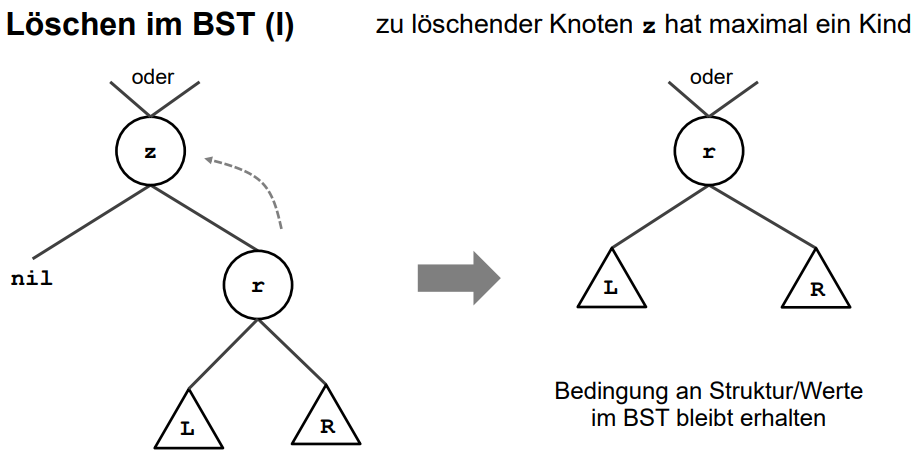
\includegraphics[width=9cm]{pictures/binärerSuchbaumLöschen1.PNG}
                        \item[] 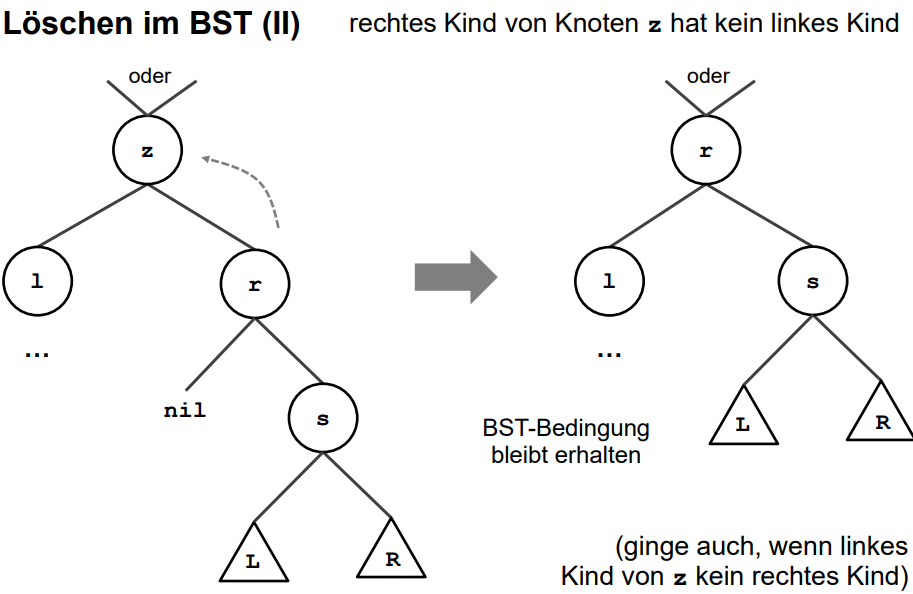
\includegraphics[width=9cm]{pictures/binärerSuchbaumLöschen2.PNG}
                        \item[] 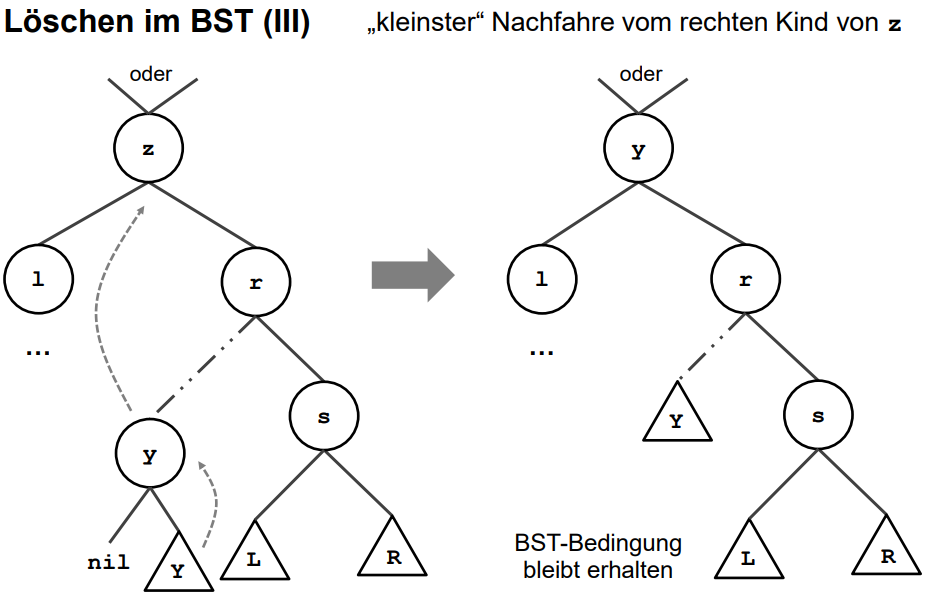
\includegraphics[width=9cm]{pictures/binärerSuchbaumLöschen3.PNG}
                    \end{itemize}
                    \clearpage
              \item \textit{Code}
              \item[]\index{transplant}
                        \begin{codeBlock}[autogobble]{title={transplant(T,u,v) // Hängt Teilbaum v an Parent von u}}
                            IF u.parent == nil THEN
                                T.root = v;
                            ELSE
                                IF u == u.parent.left THEN
                                    u.parent.left = v;
                                ELSE
                                    u.parent.right = v;
                            IF v != nil THEN
                                v.parent = u.parent;
                        \end{codeBlock}
                        \begin{codeBlock}[autogobble]{title={delete(T,z)}}
                            IF z.left == nil THEN
                                transplant(T,z,z.left)
                            ELSE
                                IF z.right == nil THEN
                                    transplant(T,z,z,left)
                                ELSE
                                    y = z.right;
                                    WHILE y.left != nil DO y = y.left;
                                    IF y.parent != z THEN
                                        transplant(T,y,y.right)
                                        y.right = z.right;
                                        y.right.parent = y;
                                    transplant(T,z,y)
                                    y.left = z.left;
                                    y.left.parent = y;
                        \end{codeBlock}
              \item Laufzeit = $O(h)$
              \item Laufzeit ist damit besser, wenn viele Suchoperationen und $h$ klein relativ zu $n$
          \end{itemize}
\clearpage
    \item \fatsf{Höhe eines BST}
          \begin{itemize}
              \item \textit{Best Case:}
                    \begin{itemize}
                        \item Vollständiger Baum (Alle Blätter gleiche Tiefe)
                        \item $h = O(log_2 n)$
                        \item Laufzeit = $O(log_2 n)$
                    \end{itemize}
              \item \textit{Worst Case:}
                    \begin{itemize}
                        \item Degenerierter Baum (links- bzw. rechtslastiger Baum)
                        \item $h = n - 1$
                        \item Laufzeit = $\Theta(n)$
                    \end{itemize}
              \item \textit{Durchschnittliche Höhe:}
                    \begin{itemize}
                        \item Erwartete Höhe: $\Theta(log_2 n)$
                    \end{itemize}
          \end{itemize}
    \item \fatsf{Suchbäume als Suchindex}\index{Suchindex}
          \begin{itemize}
              \item Knoten speichert nur Primärschlüssel und Zeiger auf Daten
              \item Zusätzliche Indizes möglich, kosten aber Speicherplatz
              \item[] 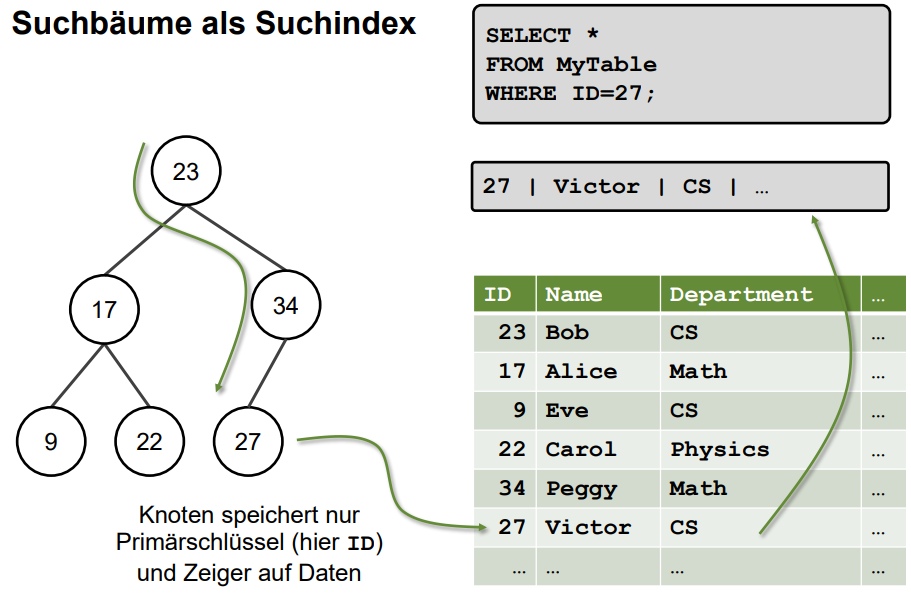
\includegraphics[width=12cm]{pictures/suchbaumSuchindex.PNG}
          \end{itemize}
\end{itemize}
\pagebreak
\end{document}
